\chapter{Emulátory prevádzky SCADA systémov}
\label{porovnanie}
\tab V tejto kapitole uvediem základný prehľad a porovnanie bežne používanych monitorovacích a emulačných nástrojov pre protokoly IEC 60870-5-104 a IEC 60870-5-104. Programy, ktorým sa budem venovať, slúžia nielen na~monitorovanie komunikácie reálnych IEC 60870-5-104 a DLMS/COSEM meracích zariadení, ale aj na ich emuláciu. Popis inštalácie jednotlivých programov je uvedený v prílohe \ref{Ako}.
\section{IEC 60870-5-104 - DLMS/COSEM}
\subsection{DMLS Director}
\textbf{Výrobca:} Firma GuruX Ltd. je fínska spoločnosť špecializujúca sa na protokol DLMS využívaný v inteligentných meračoch\footnote{GuruX Ltd. \url{http://www.gurux.fi} [Online: Október 2017]}. Firma poskytuje produkty pre automatické zaznamenávanie hodnôt z meracích zariadení a umožnuje tým vytvorenie vlastných AMR systémov (systémov pre automatickú správu meracích zariadení). \par
\noindent \textbf{Popis produktu:} DLMS Director je open source software navrhnutý na DLMS komunikáciu a smart metering s DLMS/COSEM zariadeniami. \par 
\noindent \textbf{Protokoly:} Program DLMS Director pokrýva niekoľko komunikačných štandardov. Je zameraný na čítanie údajov a rozposielanie príkazov. Jednotlivé protokoly sú: 
\begin{itemize}
\item IEC 62056-21 Priama lokálna výmena dát
\item IEC 62056-42 Služby a procedúry pre asynchrónnu spojovú výmenu dát na fyzickej vrstve
\item IEC 62056-46 Linková vrstva využívajúca HDLC protokol
\item IEC 62056-47 COSEM transportná vrstva pre IPv4
\item IEC 62056-53 COSEM aplikačná vrstva
\item IEC 62056-61 OBIS systém na identifikáciu objektov
\item IEC 62056-62 Interface
\end{itemize} \par
\noindent \textbf{Zariadenia:} Program je schopný pracovať iba s reálnymi fyzickými zariadeniami, prípadne so zariadeniami emulovanými iným programom. Sám ich však emulovať nedokáže. So zariadeniami môže byť pripojený cez TCP/IP spojenie, terminál, alebo cez sériovú linku. \par
\noindent \textbf{Typ:} DLMS Director je open source software, ktorý je voľne dostupný na stránkach výrobcu. Zdrojové kódy sú taktiež voľne dotupné v pratričnom github repozitári\footnote{DLMS Director - zdrojové kódy \url{https://github.com/Gurux/GXDLMSDirector} [Online: Október 2017]}. \par
\noindent \textbf{Platforma:} Program je vytvorený pre OS Windows. Na iných platformách s ním nie je možné pracovať. \par
\noindent \textbf{Prípadová štúdia:} Program samotný slúži ako jedna klientská stanica umožňujúca pripojenie niekoľkých meracích zariadení. Pri pridávaní nového zariadenia je možnosť nastavenia jednotlivých parametrov spolu s preddefinovanými hodnotami. Ukážka pridania nového zariadenia je na obrázku \ref{DLMSConf}. 
\begin{figure}[h]
    \centering
    \scalebox{0.8}{\includegraphics{DLMSdirectorConf.png}}
    \caption{Konfigurácia nového zariadenia v programe DLMS Director}
\label{DLMSConf}
\end{figure}
Odkaz na popis konfigurácie rôznych zariadení je medzi prílohami, časť \ref{Ako_DLMS}. Po pripojení k serveru zobrazí program zoznam všetkých objektov, ktoré server obsahuje. Objekty sú rozdelené do množín podľa ich typu, napr. {\tt Data, Register, Clock, MacAddress Setup}. Ukážka je na obrázku \ref{DLMS_List}.
\begin{figure}[h]
    \centering
    \scalebox{0.55}{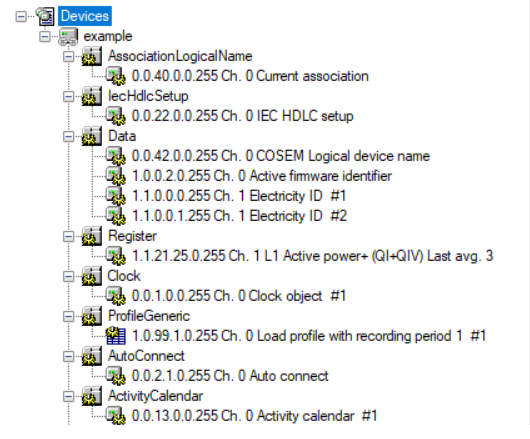
\includegraphics{DLMS_List.png}}
    \caption{Zoznam pripojených objektov}
\label{DLMS_List}
\end{figure}
Je možné čítať hodnoty atribútov jednotlivých objektov, avšak iba všetkých hodnôt naraz. Nie je možné odoslať samostatný príkaz na prečítanie napríklad logického mena objektu. Je tiež možné prečítať hodnoty celej skupiny objektov v jednom príkaze, ale iba v rámci jedného typu. Napríklad hodnoty objektov typu {\tt Data}. \par
Pri testovaní bola použitá knižnica v jazyku C++, ktorú poskytuje spoločnosť GuruX. Knižnica je voľne k dispozícií v Github repozitári\footnote{DLMS knižnica - Github \url{https://github.com/Gurux/Gurux.DLMS.cpp} [Online: Marec 2018]} a umožňuje vytvorenie vlastných aplikácií pre DLMS. Spolu s knižnicou sú k dispozícií vzorové programy pre klienta a server. Programy sú vytvorené pre OS Linux. Návod na inštaláciu knižnice je medzi prílohami \ref{kniznica}. Vzorový program servera vytvorí pri spustení štyri rôzne DLMS servery:
\begin{itemize}
\item port 4060 - DLMS server využívajúci krátke mená (Short Names - SN)
\item port 4061 - DLMS server využívajúci logické mená (Logical Names - LN) 
\item port 4062 - DLMS server využívajúci krátke mená spolu s protokolom IEC 62056-47
\item port 4063 - DLMS server využívajúci logické mená spolu s protokolom IEC 62056-47
\end{itemize} \par
Samotné testovanie pozostávalo vo vytvorení spojenia medzi programom DLMS Director a vzorovým programom pre server. Program bol ale čiastočne upravený aby bol užívateľsky o niečo prívetivejší a aby podporoval väčšiu škálu možností. Po spustení sa vytvorí iba jeden server na porte 4060 využívajúci logické mena. Bola pridaná možnosť hodnoty vzdialene meniť, nie iba čítať a bola pridaná možnosť využívať autentizáciu heslom typu {\tt low}. Zmenený program bol umiestnený na github repozitár\footnote{GitHub \url{https://github.com/janpristas/bakalarska-praca}}. Na jeho úspešnú kompiláciu a spustenie je potrebné mať nainštalovanú vyššie spomínanú knižnicu. \par
Vytvorenie spojenia a testovanie pozostávalo z niekoľkých krokov:
\begin{enumerate}
\item Bol spustený DLMS Director a program servera. Server nebolo nutné nijako ďalej konfigurovať. Bolo možné sa s ním priamo spojiť.
\item V DLMS Directore bolo potrebné nakonfigurovať server s ktorým sa ide program spojiť:
\begin{enumerate}
\item {\tt File} $\rightarrow$ {\tt Add Device}
\item Zvoliť meno pre server
\item Zvoliť výrobcu $\rightarrow$ {\tt Gurux}, 
\item Zvoliť autentizáciu $\rightarrow$ {\tt Low} a heslo $\rightarrow$ {\tt password} (nastavené v programe servera)
\item Nastaviť IP adresu servera a port 4060
\end{enumerate}
\item Po úspešnom nakonfigurovaní bolo možné vytvoriť spojenie so serverom. Spojenie inicializuje program DLMS Director. V ľavom paneli bolo potrebné rozkliknúť zoznam {\tt Devices} a kliknúť pravým tlačítkom na server, následne na {\tt Connect}.
\item Po vytvorení spojenia sa zobrazil zoznam pripojených zariadení, z ktorých bolo možné čítať a zapisovať hodnoty, príkazy {\tt Read} a {\tt Write}.
\end{enumerate} \par
Testovaciu topológiu je možné vidieť na obrázku \ref{dlmstopology}.
\begin{figure}[h]
    \centering
    \scalebox{0.8}{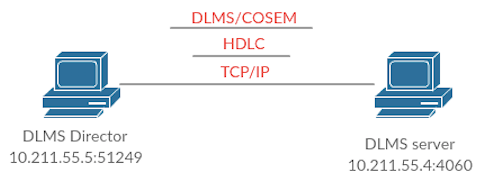
\includegraphics{dlms_topology}}
    \caption{Ukážka testovacej topológie pre program DLMS Director}
\label{dlmstopology}
\end{figure}
Testovací server obsahoval niekoľko rôznych objektov. Testovanie spočívalo v dotazovaní sa na hodnoty atribútov týchto objektov. Objekty boli napríklad typu {\tt Data, Clock, SapAssigment, ActivityCalendar}. Komunikácia bola zachytená pomocou nástroja Wireshark a bol vytvorený súbor DLMSDirector.pcap uložený v github repozitári. \footnote{GitHub \url{https://github.com/janpristas/bakalarska-praca}} \par
\noindent \textbf{Zhrnutie:} DLMS Director je dobre spracovaný program určený hlavne na čítanie údajov a riadenie meracích zariadení. Výhodou je, že je typu open source a možno s ním zdarma pracovať. Nevýhodou je chýbajúca možnosť emulovania koncových zariadení a tým aj prevádzky samotnej.

\subsection{XmlDemo}
\textbf{Výrobca:} iCube je švajčiarska softwarová firma zaoberajúca sa, podobne ako vyššie spomínaná firma GuruX, vývojom softwaru pre komunikačný protokol DLMS\footnote{iCube \url{https://www.icube.ch/index.html} [Online: Október 2017]}. Firma ponúka DLMS vývojové komunikačné balíky pre jazyky C++, C\# a Java, zjednodušujúce implementáciu DLMS/COSEM klientských aplikácií. Vo variante C++ sú jednotlivé komponenty implementované ako DLL, v C\# a Java variantách sú implementované ako triedy. Jednotlivé balíky ale nebudem bližšie rozoberať. \par
\noindent \textbf{Popis produktu:} XmlDemo je jednoduchý DLMS "čítač"\ hodnôt uložených v DLMS/COSEM meracích zariadeniach. Implementácia využíva vyššie spomenuté DLMS balíky, konkrétne komponenty {\tt xmlpdu} na výstup vo formáte xml, {\tt ezhdlc} pri vyžití HDLC spojenia a {\tt wrapper} pri spojení cez TCP/IP. Program XmlDemo je v úlohe klienta, ktorý zasiela žiadosti serveru (zariadeniam) a prijíma odpovede. Napríklad, klient pošle žiadosť {\tt read the object 1.0.1.8.0.255} a server odpovie {\tt 1789.8 kWh}. \par
\noindent \textbf{Protokoly:} Program je vytvorený na komunikáciu so zariadeniami pomocou protokolu DLMS/COSEM. \par
\noindent \textbf{Zariadenia:} Program je schopný pracovať iba s reálnymi fyzickými zariadeniami, prípadne so zariadeniami emulovanými iným programom. Sám ich emulovať nedokáže. Podporuje komunikáciu medzi zariadeniami a aplikáciou cez TCP/IP a HDLC. \par
\noindent \textbf{Typ:} XmlDemo je zdarma poskytovaný program spoločnosťou iCube, nakoľko sa jedná o ukážku programu vytvoreného vo vyššie spomínaných vývojových balíkoch. \par
\noindent \textbf{Platforma:} Obdobne ako predchádzajúci program je aj XmlDemo prispôsobený iba na OS Windows. Na obrázku \ref{XmlDemo} je ukážka užívateľského rozhrania. Spôsob prijímania správ a logovací záznam vo formáte xml je na obrázku \ref{XmlDemo-term}. \par
\begin{figure}[h]
	\centering
    \scalebox{0.48}{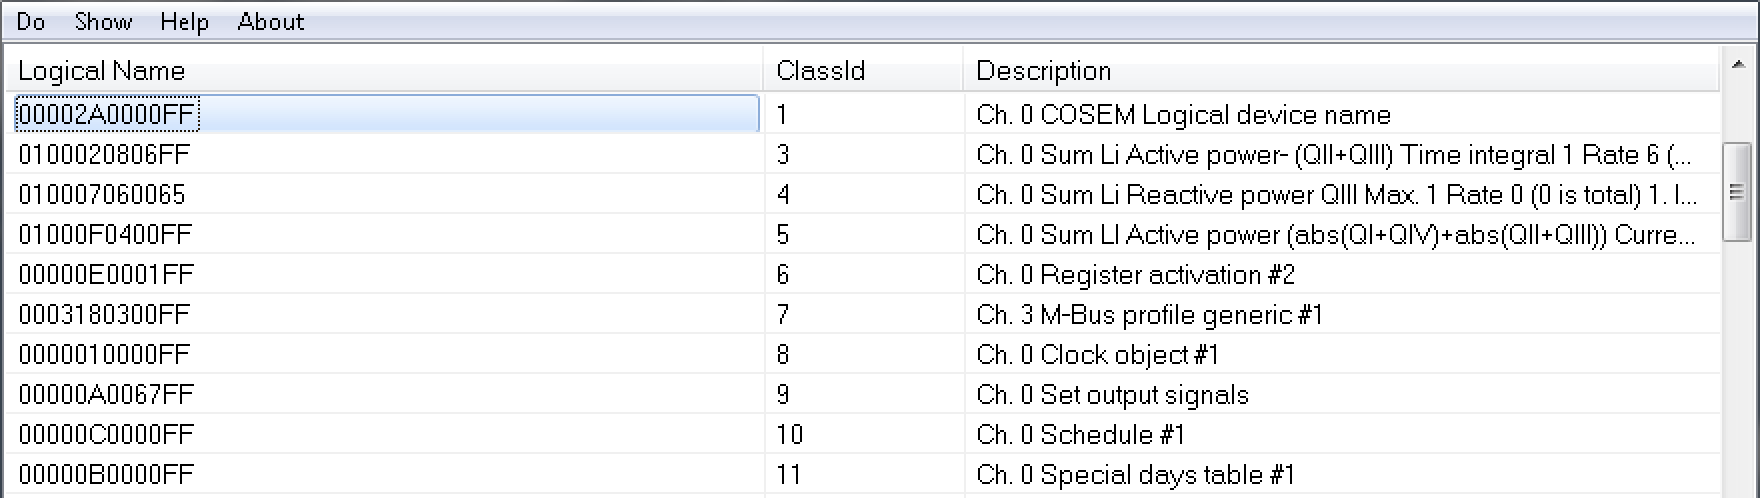
\includegraphics{XMLDemo}}
    \caption{Užívateľské rozhranie XmlDemo}
\label{XmlDemo}
\end{figure} \par

\begin{figure}[h]
    \centering
    \scalebox{0.6}{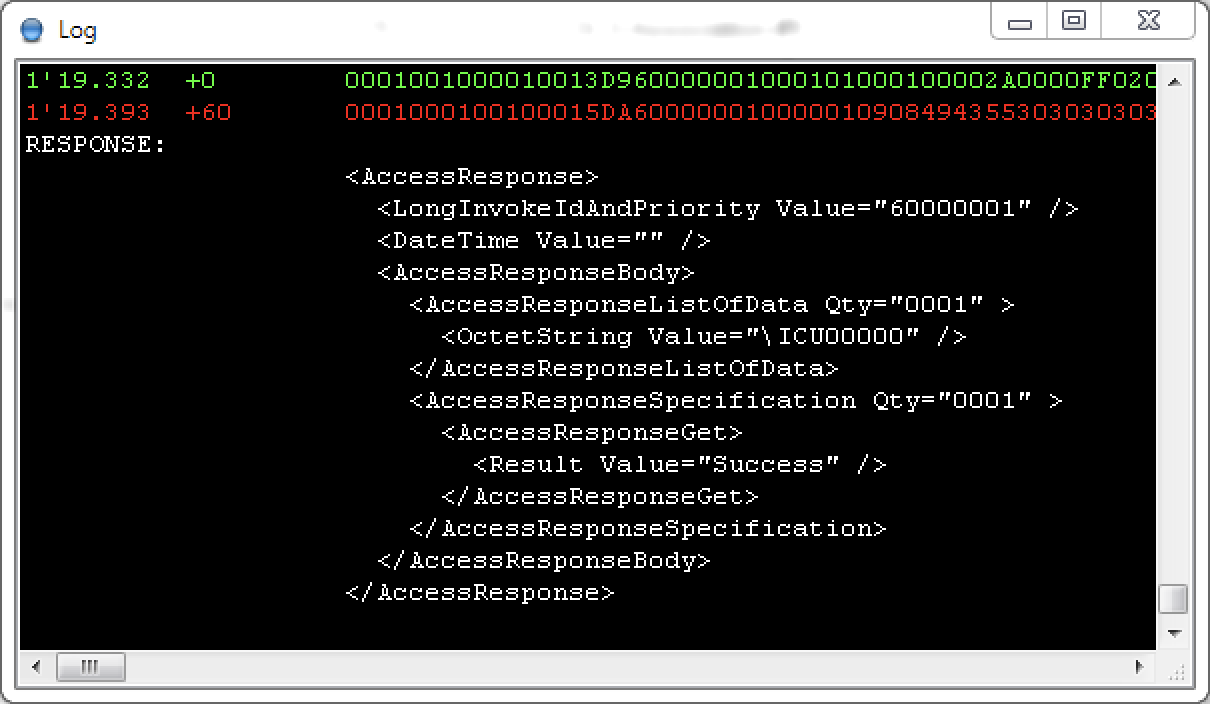
\includegraphics{XMLDemo-terminal}}
    \caption{Užívateľské rozhranie XmlDemo}
\label{XmlDemo-term}
\end{figure} \par
\noindent \textbf{Prípadová štúdia:} Čo sa topológie týka, program funguje ako vyššie popísaný DLMS Director. Program samotný slúži ako klientská stanica, ku ktorej je možné pripojiť jednotlivé monitorovacie zariadenia. \par
Pri testovaní bol použitý vzorový program pre server komunikujúci na porte 4063 využívajúc spojenie cez TcpUdp. Program XmlDemo síce umožňuje komunikáciu so serverom cez HDLC, avšak iba ak sú zariadenia prepojené cez sériovú linku. To som však nemal pri testovaní možnosť vyskúšať, nakoľko som nemal k dispozícií reálne fyzické zariadenie. \par
Vytvorenie spojenia medzi klientom a serverom opäť pozostávalo z niekoľkých krokov:
\begin{enumerate}
\item Bol spustený program XmlDemo a pôvodný vzorový program servera, neobsahújúci nijaké zmeny. 
\item Bolo potrebné nakonfigurovať program XmlDemo:
\begin{enumerate}
\item {\tt Show} $\rightarrow$ {\tt Settings}
\item {\tt Select TCP profile}
\item Nastaviť IP adresu servera a port 4063
\item Nastaviť referenčný model $\rightarrow$ {\tt LN}
\item Nastaviť timeout, obe hodnoty {\tt Connect} a {\tt Response} na prijateľné hodnoty v milisekundách, v našom prípade 1000
\item Nastaviť adresy pre klienta aj server, v našom prípade obe na 0
\end{enumerate}
\item Po nakonfigurovaní bolo možné vytvoriť spojenie. {\tt Do} $\rightarrow$ {\tt Connect} a {\tt Do} $\rightarrow$ {\tt Read object-list}.
\end{enumerate} \par
Testovacia topológia je obdobná ako pri testovaní programu DLMS Drector. Je možné ju vidieť na obrázku \ref{xmldemotopology}.
\begin{figure}[h]
    \centering
    \scalebox{0.8}{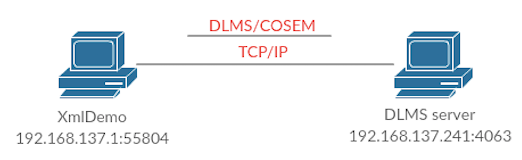
\includegraphics{xmldemo_topology}}
    \caption{Ukážka testovacej topológie pre program XmlDemo}
\label{xmldemotopology}
\end{figure}
 Po vytvorení spojenia medzi klientom a serverom, program (XmlDemo) automaticky zobrazí zoznam všetkých pripojených objektov. Objekty sú taktiež uložené do nového .txt súboru. Zoznam je zobrazený vo formáte - {\tt logické meno | id triedy | popis}. Zápis objektu vyzerá napríklad $\rightarrow$ {\tt 0000010000FF | 8 | Ch. 0 Clock object \#1}. Následne je možné z jednotlivých objektov čítať hodnoty atribútov. Je možné čítať hodnoty iba vybraných atribútov, na rozdiel od programu DLMS Director, ktorý umožňuje iba čítanie všetkých hodnôt daného objektu naraz. Po kliknutí na jednotlivé objekty sa zobrazí zoznam ich atribútov. Po kliknutí na jednotlivé atribúty sa prečíta ich hodnota. Testovanie prebiehalo obdobne ako pri programe DLMS Director. Komunikácia bola zachytená nástrojom Wireshark a bol vytvorený súbor XmlDemo.pcap uložený v github repozitári. \footnote{GitHub \url{https://github.com/janpristas/bakalarska-praca}} \par
\noindent \textbf{Zhrnutie:} Čo sa týka samotnej funkcionality, poskytuje program obdobné funkcie a možnosti ako program DLMS Director, avšak hlavnou nevýhodou je absencia komunikácie pomocou HDLC cez IP vrstvu. Je to možné iba na fyzickej vrstve. Na testovacie účely je preto vhodnejší program DLMS Director. XmlDemo taktiež ponúka o niečo horšie GUI, v ktorom sa nepracuje tak dobre a intuitívne ako v DLMS Directore.

\section{IEC 60870-5-104}
\subsection{WinPP104}
\textbf{Výrobca:} Firma Berthold Boeser Ingenieurbüro je nemecká spoločnosť, ktorá vyvíja a distribuje testovacie programy pre protokoly diaľkového riadenia\footnote{Berthold Boeser Ingenieurbüro \url{http://www.ppfink.de//} [Online: Október 2017]}. Jednotlivé protokoly sú: 
\begin{itemize}
\item IEC: 60870-5-101, 60870-5-102, 60870-5-103, 60870-5-104
\item AEG: GEADAT 81, GEATRANS F202, F203, F220, F202KC, SEAB 1-F/N, PMF234C
\item BBC: ZM20, I21
\item Landis\&Gyr: TELEGYR 800
\item Mauell: ME 8008, 8018 PDM
\item SAT: 1703 PCM
\item SEL: ZPC3600/SPC17
\item Siemens: SINAUT ST1, 4-FW, SINAUT 8-FW DPDM, SINAUT 8-FW PCM, FW 517/535/537, EFD 400, SAS/Z70
\end{itemize} \par
\noindent \textbf{Popis produktu:} WinPP104 je testovací a emulačný nástroj pracujúci nad protokolom IEC 60870-5-104. Okrem bežnej komunikácie tiež umožňuje odosielanie a prijímanie správ iba simulovať a tým sledovať rôzne faktory ako napr. oneskorenie príkazu. Výsledný záznam komunikácie sa dá exportovať do .csv súboru. Program rovnako umožňuje záznamy z .csv súborov aj nahrávať a následne ich spracovať. \par
\noindent \textbf{Protokoly:} Program je uspôsobený na komunikáciu výhradne nad protokolom IEC 60870-5-104. \par
\noindent \textbf{Zariadenia:} WinPP104 umožňuje sledovať reálne fyzické meracie zariadenia, ale aj vytvorenie vlastného klienta alebo servera pre simulačné účely. Prepojenie medzi zariadeniami je možné cez LAN alebo TCP/IP. \par
\begin{figure}[H]
    \centering
    \scalebox{0.35}{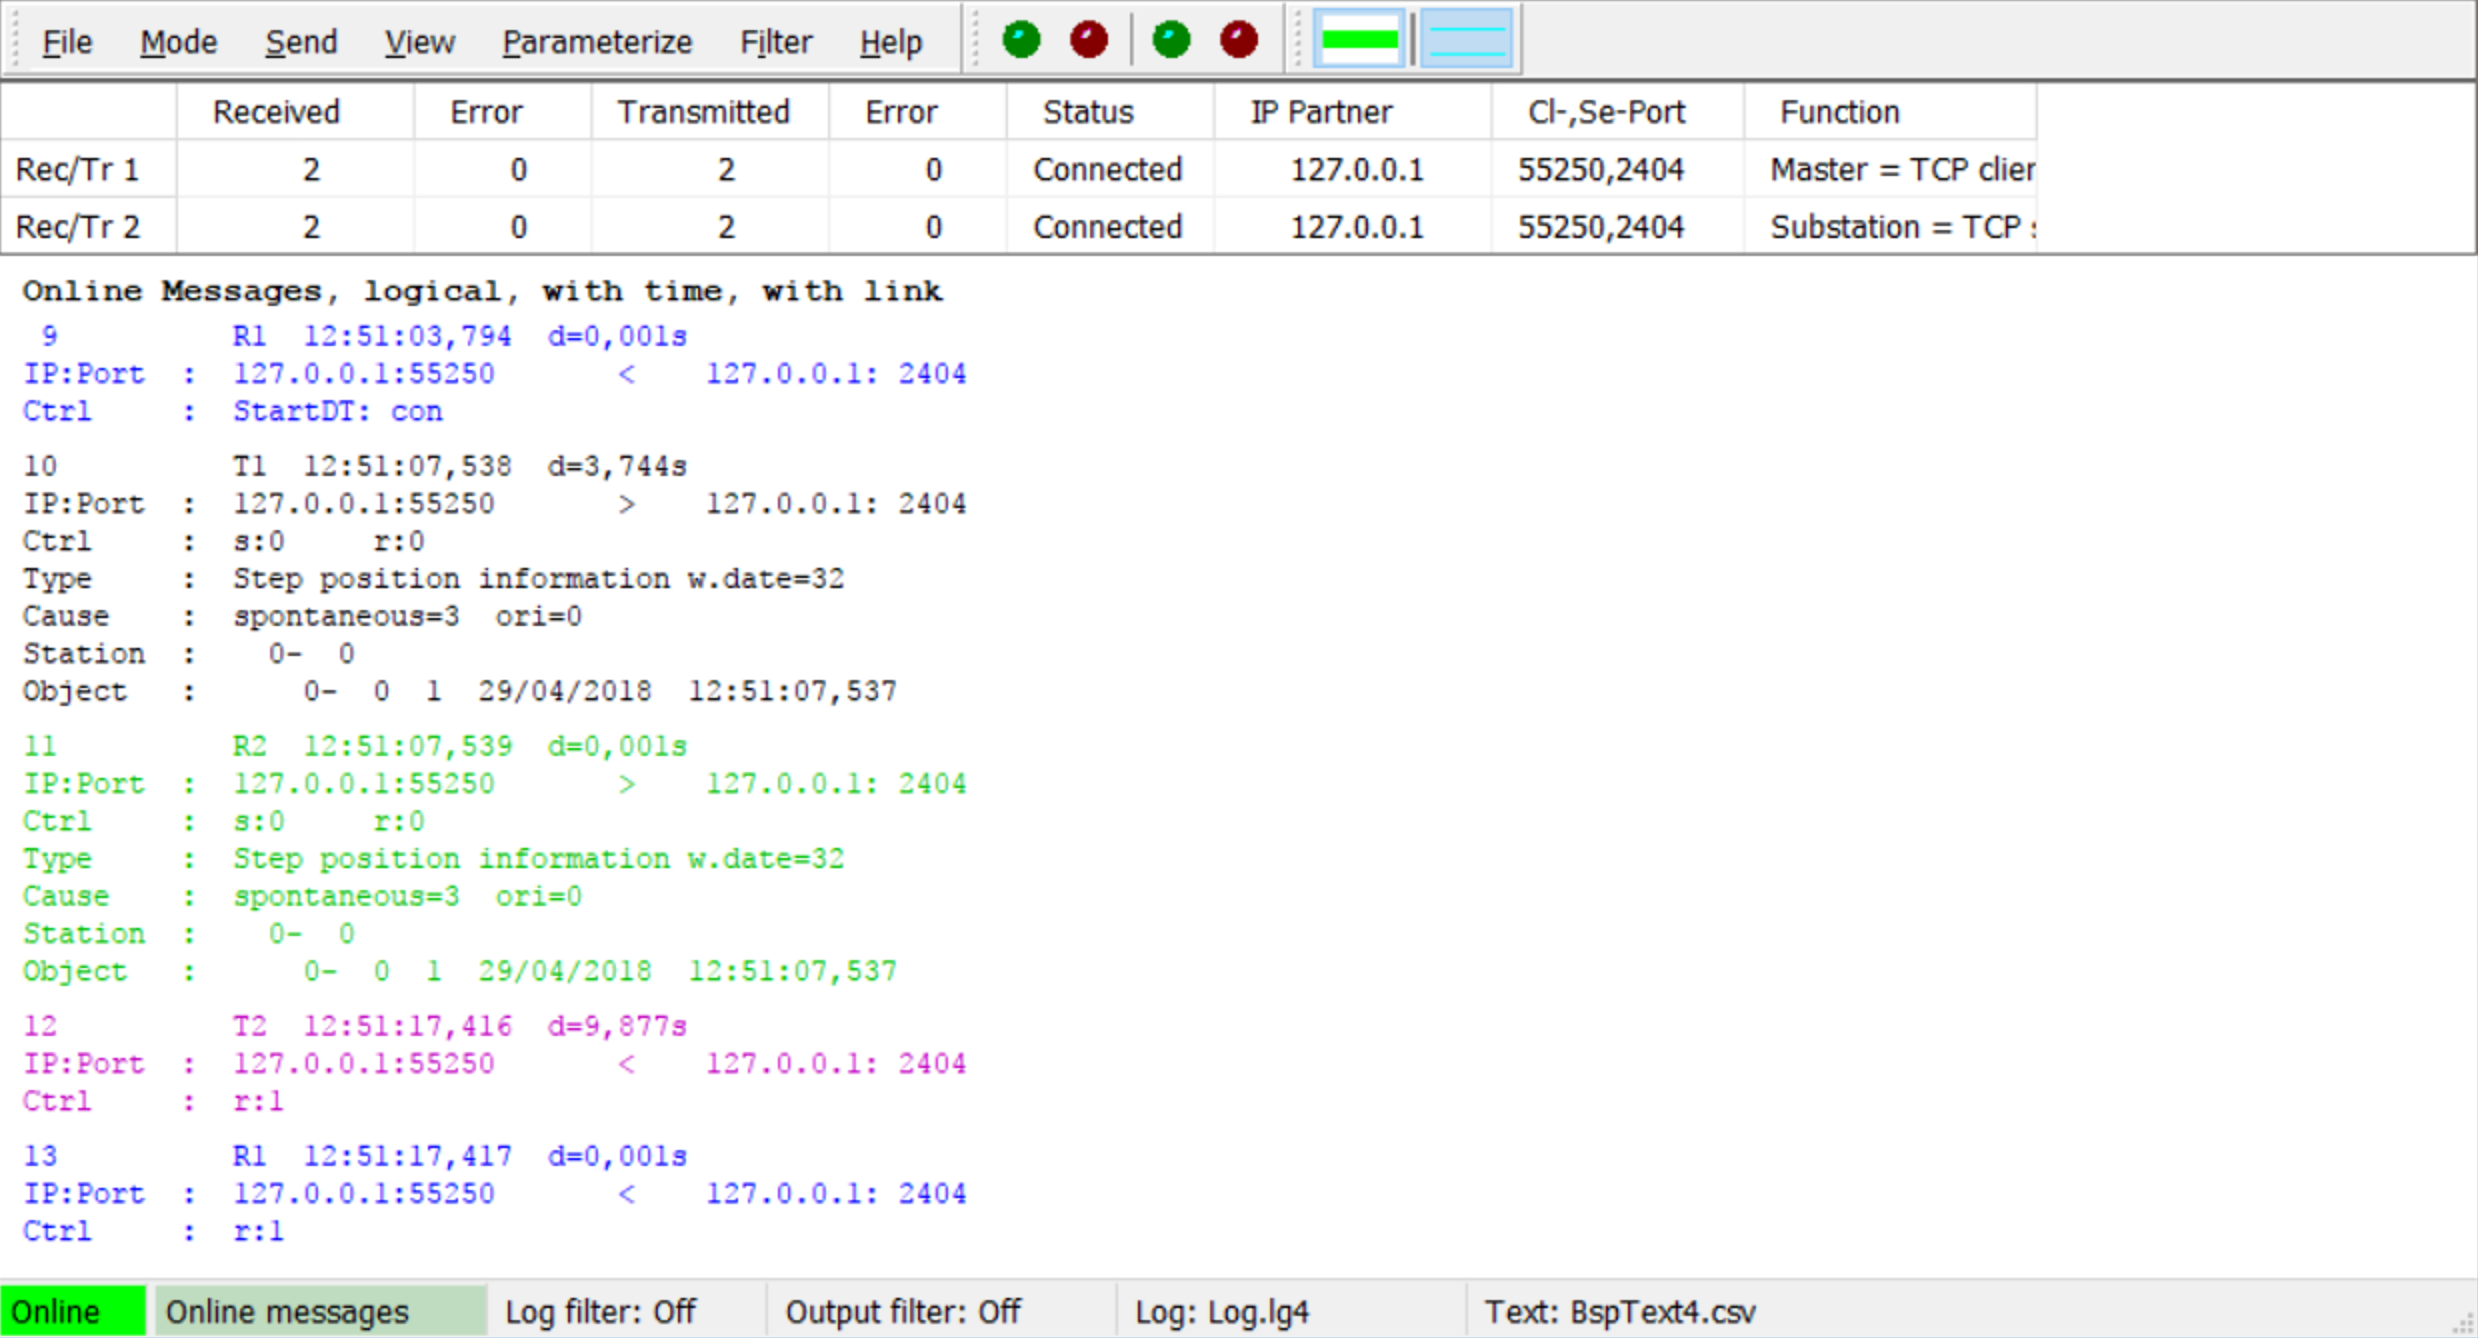
\includegraphics{WinPP104}}
    \caption{Užívateľské rozhranie WinPP104}
\label{WinPP104}
\end{figure}
\noindent \textbf{Typ:} Výrobca poskytuje zdarma demo verziu, ktorá má však určité obmedzenia. Pri každom spustení aplikácie je nutné si celý systém nanovo nastavovať, naše predošlé nastavenia nebudú uložené. Navyše je možné prijať a odoslať iba 20 správ, čo striktne zamedzí dlhodobému monitorovaniu systému. \par
\noindent \textbf{Platforma:} Program je vytvorený na platformu OS Windows. Na obrázku \ref{WinPP104} je ukážka užívateľského rozhrania programu WinPP104, konkrétne ide o ukážku pripojenia zariadení cez TCP/IP a o ich monitorovanie. \par
\noindent \textbf{Prípadová štúdia:} WinPP104 umožňuje v rámci jedného spustenia vytvorenie jednej stanice klienta a jednej stanice servera. Je ale možné program spustiť niekoľkokrát a emulovať niekoľko klient/server spojení. Pri vytváraní nového uzlu poskytuje program defaultné nastavenia, ktoré je možné vidieť na obrázku \ref{WinPP104Conf}.
\begin{figure}[h]
    \centering
    \scalebox{0.5}{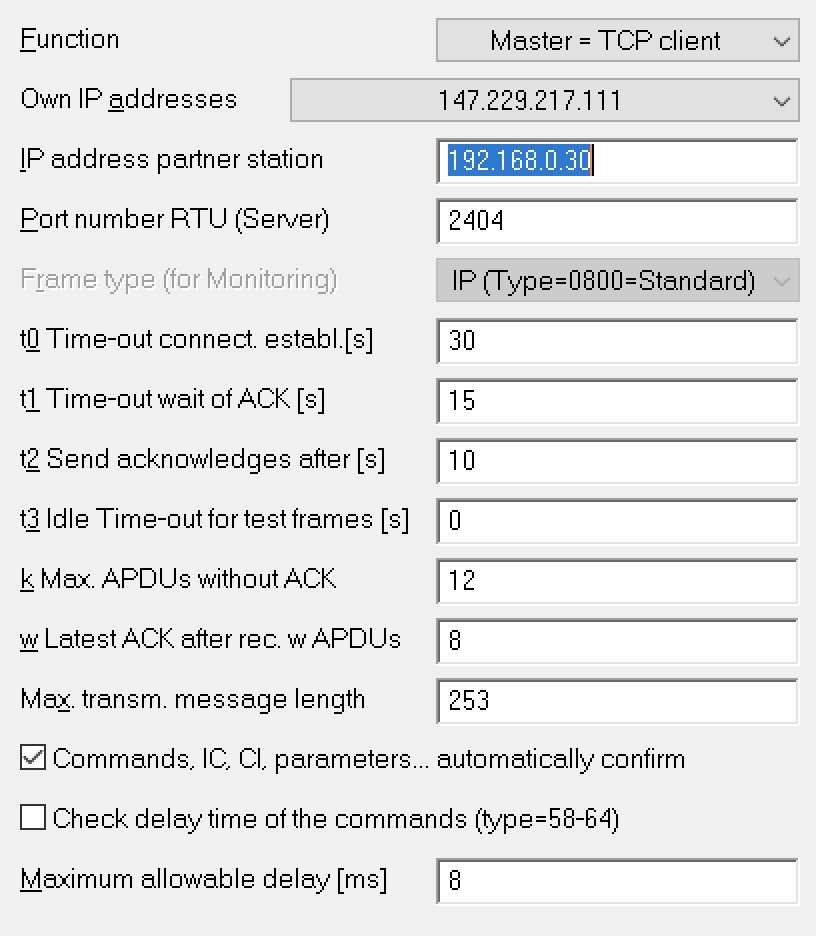
\includegraphics{WinPP104C}}
    \caption{Konfigurácia nového objektu}
\label{WinPP104Conf}
\end{figure} \par
Vytvorenie testovacieho prostredia pozostávalo z niekoľkých častí:
\begin{enumerate}
\item Spustenie programu WinPP104
\item Konfigurácia nového uzlu klienta:
\begin{enumerate}
\item {\tt Parameterize} $\rightarrow$ {\tt Receiver/Transmitter 1}
\item {\tt Function} = {\tt Master = TCP Client}
\item {\tt IP address partner station} = 127.0.0.1
\item {\tt Port number RTU (Server)} = 2404
\item Zvyšné parametre mali defaultné hodnoty
\item {\tt OK}
\end{enumerate}
\item Konfigurácia nového uzlu servera:
\begin{enumerate}
\item {\tt Parameterize} $\rightarrow$ {\tt Receiver/Transmitter 2}
\item {\tt Function} = {\tt Substation = TCP Server}
\item {\tt IP address partner station} = 127.0.0.1
\item {\tt Port number RTU (Server)} = 2404
\item Zvyšné parametre mali defaultné hodnoty
\item {\tt OK}
\end{enumerate}
\item {\tt Mode} $\rightarrow$ {\tt Online}, následné sa vytvorilo spojenie medzi jednotlivými uzlami a bolo možné zasielať príkazy
\end{enumerate}
Pri samotnej komunikácií poskytuje program 12 preddefinovaných správ a 12 zoznamov. Je možné ich dodatočne prekonfigurovať podľa potreby:
\begin{itemize}
\item {\tt Parameterize} $\rightarrow$ {\tt Messages} $\rightarrow$ 1,2,3,...
\item {\tt Parameterize} $\rightarrow$ {\tt Lists} $\rightarrow$ 1,2,3,...
\end{itemize}
Je možné nastaviť napr. typ správy, dôvod (cause) odoslania správy, zdrojovú, cieľovú adresu a pod. Ukážka konfigurácie správy je na obrázku \ref{WinPP104Mess}.
\begin{figure}[h]
    \centering
    \scalebox{0.5}{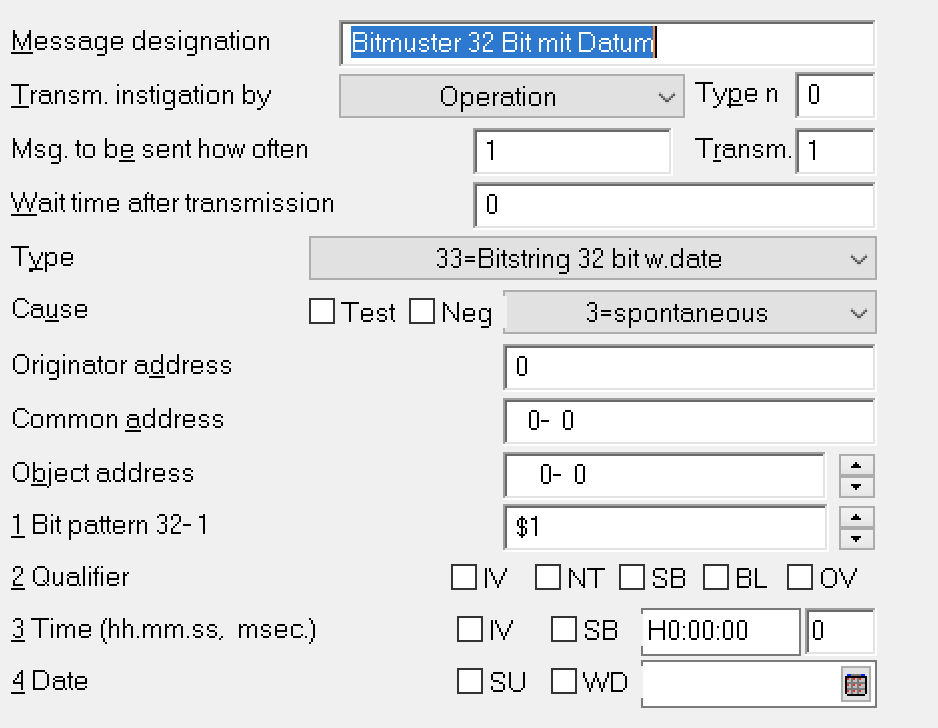
\includegraphics{WinPP104M}}
    \caption{Konfigurácia novej správy}
\label{WinPP104Mess}
\end{figure} \par
Zasielanie správ alebo zoznamov je možné cez {\tt Send} $\rightarrow$ {\tt Messages}/{\tt Lists} $\rightarrow$ 1,2,3,... \par
Testovanie pozostávalo vo vytvorení jednoduchej topológie a v zaslaní/prijatí niekoľkých preddefinovaných správ aby sa overilo, či komunikácia odpovedá štandardom protokolu IEC 60870-5-104. Ukážka testovacej topológie je na obrázku \ref{WinPP104-Topology}.
\begin{figure}[h]
    \centering
    \scalebox{0.8}{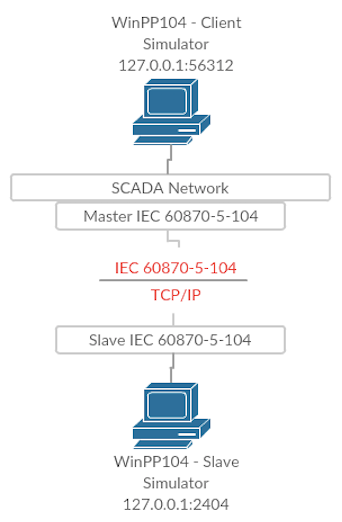
\includegraphics{WinPP104-Topology}}
    \caption{WinPP104 - Testovacia topológia}
\label{WinPP104-Topology}
\end{figure}
Program bol spustení na jednom zariadení a komunikácia bola zachytená nástrojom RawCap na rozhraní loopback. Z komunikácie bol vytvorený .pcap súbor WinPP104.pcap uložený v github repozitári \footnote{GitHub \url{https://github.com/janpristas/bakalarska-praca}}. Z následnej analýzy odchytených dát bolo overené, že komunikácia bola validná a odpovedala protokolu IEC 104.
\begin{figure}[H]
    \centering
    \scalebox{0.4}{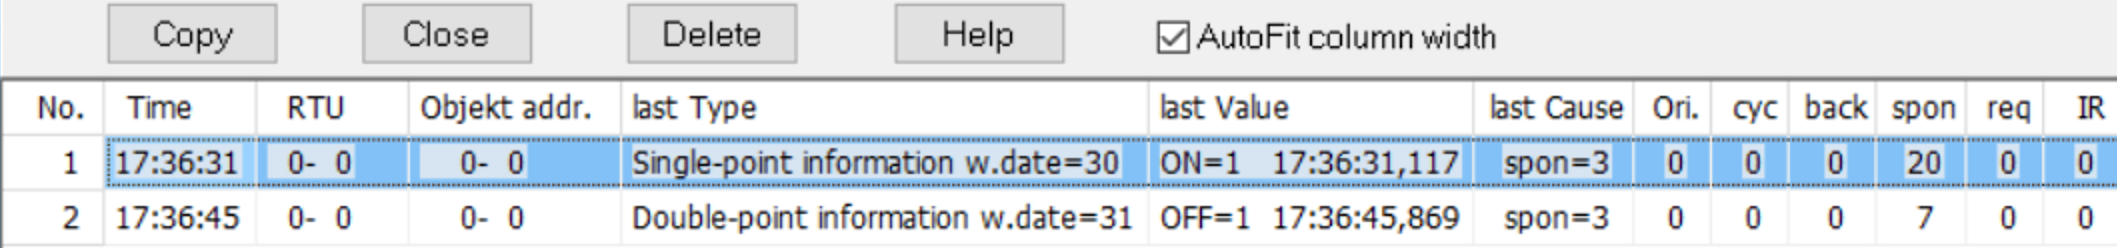
\includegraphics{WinPP104-PI}}
    \caption{Obraz procesov programu WinPP104}
\label{ProcessImage}
\end{figure} \par
\noindent \textbf{Zhrnutie:} WinPP104 je veľmi dobre vytvorený emulačný a monitorovací nástroj. Veľkou výhodou je, že dokáže jednotlivé zariadenia aj emulovať. 
Navyše pri monitorovaní alebo emulovaní zariadenia program automaticky vytvára tzv. obraz procesov (process image) o jednotlivých zariadeniach a komunikácii s nimi. Obraz procesov je dobrý na rýchly prehľad stavu jednotlivých objektov. Tiež je možné vyfiltrovať iba určitú komunikáciu podľa nami zadaného filtra. Ukážka je na obrázku \ref{ProcessImage}. Obraz procesov je možné zobraziť cez {\tt View} $\rightarrow$ {\tt Process image}. \par
\noindent Počas behu programu vytvára systém tabuľku jednotlivých komunikácií, nazývanú tiež tabuľka TCP 104, viď obrázok \ref{WinPP104-TCP}. TCP 104 tabuľka je vhodná na rýchly prehľad aktívnych spojení, na filtrovanie spojení a sledovanie napr. nezabezpečených spojení (cez WiFi) alebo zariadení, ktoré sa nechovajú podľa očakávaní. \par
\begin{figure}[h]
    \centering
    \scalebox{0.4}{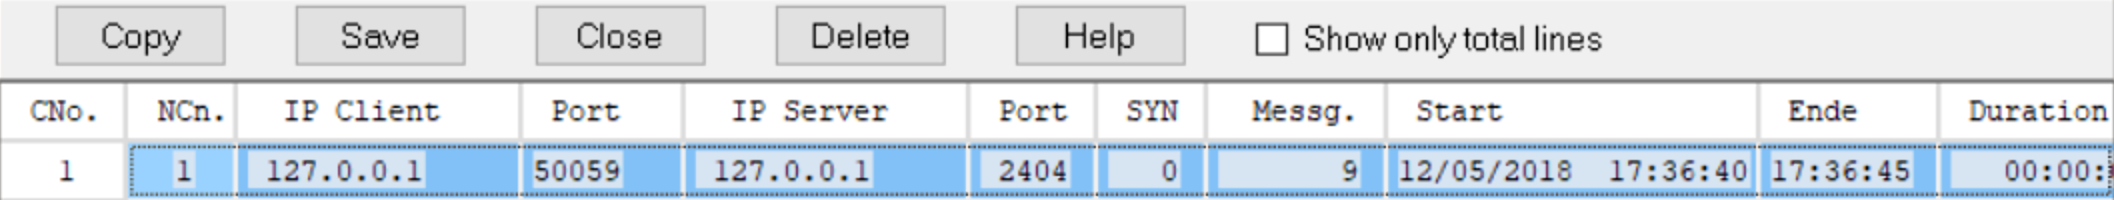
\includegraphics{WinPP104-TCP}}
    \caption{Prehľad TCP spojení programu WinPP104}
\label{WinPP104-TCP}
\end{figure}
\noindent Nevýhodou však zostáva, že program je voľne dostupný iba v rámci demoverzie, ktorá neumožňuje uloženie konfigurácií systému a je možné zaslanie a prijatie iba 20 správ medzi uzlami. Toto obmedzenie značne komplikuje konfiguráciu a dlhodobé sledovanie rozsiahlejších systémov. Taktiež je práca s programom relatívne komplikovaná a prvotné zorientovanie sa v systéme je o to náročnejšie. Pre porovnanie, nie je také intuitívne ako napr. v programoch Client/Server Simulator, ktoré budú popísané v predposlednej podkapitole.

\subsection{Knižnica OpenMUC - j60870}
\textbf{Výrobca:} OpenMUC je framework založený na jazyku Java a OSGi (špecifický interface pre jazyk Java), ktorý umožňuje jednoduchší vývoj špecifických monitorovacích, zaznamenávacích a riadiacich systémov. Framework bol vytvorený na Fraunhoferovom inštitúte pre solárne energetické systémy vo Freiburgu. Podporuje vývoj softwaru pre niekoľko komunikačných protokolov, napr.: \par
\begin{itemize}
\item M-Bus
\item IEC 61850 
\item IEC 62056-21
\item IEC 60870-5-104
\end{itemize} \par
\noindent \textbf{Popis produktu:} OpenMUC - j60870 je knižnica pre jazyk Java JDK\footnote{OpenMUC - j60870 \url{https://www.openmuc.org/openmuc/} [Online: Október 2017]}. Umožňuje vytvorenie (naprogramovanie) koncových staníc typu klient/server. Výsledný program môže slúžiť ako emulačný prostriedok ale aj ako reálne monitorovacie zariadenie. Vytvorené simulačné programy monitorovacích/meracích zariadení by podľa špecifikácie výrobcu mali byť schopné komunikovať s akýmkoľvek zariadením využívajúcim protokol IEC 60870-5-104. \par
\noindent \textbf{Protokoly:} Knižnica implementuje komunikačný štandard IEC 60870-5-104. \par
\noindent \textbf{Zariadenia:} Po naprogramovaní vlastného programu klient/server je možné pripojiť alebo sa pripojiť k reálnemu fyzickému IEC monitorovaciemu/meraciemu zariadeniu, prípadne k zariadeniam emulovaným iným programom. \par
\noindent \textbf{Typ:} Knižnica j60870 je licencovaná pod GPLv3. Je možné si od výrobcu zakúpiť proprietárnu licenciu. \par
\noindent \textbf{Platforma:} S knižnicou je možné pracovať pod OS Windows alebo pod akýmkoľvek UNIX-like OS. Ja osobne som s knižnicou pracoval pod Mac OSX. Bohužiaľ nie je k dispozící nijaké GUI, ani vývojové prostredie na vytvorenie vlastných zariadení, kedže ide iba o knižnicu rozširujúcu možnosti jazyka Java. \par
\noindent \textbf{Prípadová štúdia:} V rámci knižnice sú už predpripravené dva ukážkové programy, jeden pre klienta, druhý pre server. Programy sú uložené v zložke {\tt j60870/run-scripts}. Pomocou programov je ale možné vytvoriť iba jednoduché spojenie obsahujúce jedného klienta a server obsahujúci jedno koncové zariadenie. Počas testovania bola použitá rovnaká topológia ako pri programe WinPP104. Viď obrázok \ref{WinPP104-Topology}. Pre zložitejšie topológie je potrebné si naprogramovať vlastné stanice klient/server. Pri programovaní je možné využiť množstvo funkcí, ktoré knižnica poskytuje práve na takúto implementáciu. Documentáciu jednotlivých funkcií, ktoré knižnica obsahuje je možné nájsť na \footnote{JavaDoc \url{https://www.openmuc.org/iec-60870-5-104/javadoc/} [Online: Október 2017]}. V rámci testovania boli spustené oba predpripravené programy na jednom zariadení. Boli spustené v termináli (každý v samostatnom okne) daného zariadenia príkazom {\tt ./j60870-sample-server/j60870-console-client}. Program servera neumožňoval žiadnu interakciu od užívateľa, iba prijímal príkazy od klienta. V rámci programu klienta bolo možné posielať príkazy na synchronizáciu času a na čítanie hodnoty zo servera, posielať príkazy na zmenu hodnôt na servery nebolo možné. Testovanie slúžilo k preukázaniu, že programy naprogramované v knižnici j60870 sú schopné bežnej komunikacie pomocou protokolu IEC 60870-5-104. Na základe zachytenej komunikácie sa to preukázalo. Komunikácia bola zachytená pomocou nástroja Wireshark na rozhraní loopback. Bol vytvorený súbor j60870.pcap uložený v github repozitári \footnote{GitHub \url{https://github.com/janpristas/bakalarska-praca}}. \par
\noindent \textbf{Zhrnutie:} Výhodu v knižnici j60870 vidím v tom, že si užívateľ môže vytvoriť monitorovacie alebo meracie zariadenia presne na mieru, nakoľko si ich vytvorí priamo v zdrojovom kóde. Nevýhodou ale je, že práca s touto knižnicou už vyžaduje pokročilejšie znalosti a zručnosti s jazykom Java a s programovaním ako takým.

\subsection{IEC 60870-5-104 Client/Server Simulator}
\textbf{Výrobca:} FreyrSCADA \& Embedded Solution je indická spoločnosť so zameraním na vývoj softwaru pre rôzne komunikačné protokoly\footnote{FreyrSCADA \& Embedded Solution \url{http://freyrscada.com} [Online: November 2017]}. Mimo iné medzi ne patria:
\begin{itemize}
\item IEC 60870-5-101
\item IEC 60870-5-103
\item IEC 60870-5-104
\item DLMS/COSEM Client
\end{itemize}
\noindent \textbf{Popis produktu:} Vyššie uvedená spoločnosť ponúka hneď dva produkty pre protokol IEC-60870-5-104. Jeden na emuláciu klient (master) staníc a druhý na emuláciu server (slave) staníc. Každý program umožňuje emulovať až 50 uzlov klient/server a každý uzol navyše niekoľko koncových staníc. Jednotlivé nástroje umožňujú prenos dát a príkazov spolu s uložením .log správy s prehľadom aktuálnej komunikácie, ktorá na nich prebieha. Zdrojové kódy sú písané v jazyku C. \par
\noindent \textbf{Protokoly:} Oba programy sú určené na prácu výhradne nad protokolom IEC 60870-5-104. \par
\noindent \textbf{Zariadenia:} Programy si emulujú svoje vlastné koncové zariadenia, dokážu sa ale pripojiť aj k zariadeniam emulovaným iným programom, prípadne k reálnym fyzickým zariadeniam. \par
\noindent \textbf{Typ:} Program nie je open source, ale výrobca poskytuje zdarma demo verziu oboch programov. Demo verzia má však nevýhodu v tom, že po spustení má užívateľ iba 15 minút na prácu. Po uplynutí tohto času je nutné program vypnúť a spustiť znovu, spolu s opätovnou konfiguráciou klient/server staníc. Je to veľká nevýhoda, ak chcete testovať väčšiu sieť, kde iba samotné vytvorenie zaberie veľa času a na testovanie už nijaký nezostane. \par
\noindent \textbf{Platforma:} Samotné programy sú určené iba na OS Windows. Výrobca ale poskytuje aj tzv. SDK (Software Development Kit), pre klienta aj server, ktore obsahujú programy v jazyku C a umožňujú naprogramovanie koncových staníc s presnými špecifikáciami požadovanými zákazníkom. Programy SDK sú dostupné na OS Windows aj Linux. \par
\noindent \textbf{Prípadová štúdia:} Program klienta môže mať v rámci jedného uzlu pripojený iba jeden server, pričom server môže obsahovať niekoľko koncových zariadení. Je možné ale vytvoriť až 50 rôznych spojení klient/server. Pri vytváraní nového klienta/servera ponúka emulátor defaultné nastavenia, ktoré je možne vidieť na obrázku \ref{ClientConf} a \ref{ServerConf}. Prvotná konfigurácia je o niečo náročnejšia, nakoľko má program viac možností konfigurácie ako vyššie popisované programy. K dispozícií je ale niekoľko inštruktážnych videí\footnote{Tutoriály \url{http://freyrscada.com/iec-60870-5-104-Client-Simulator.php} [Online: November 2017]}, ktoré podrobne popisujú prácu s jednotlivými programami. Oba programy sú veľmi dobre spracované a umožňujú užívateľovi podrobnú konfiguráciu jednotlivých staníc podľa jeho potreby. V rámci klienta je možné nastaviť parametre ako ip adresu, port, počet pripojených staníc, adresy jednotlivých staníc a pod. V rámci servera takisto ip adresu, port, ip adresu klienta, dĺžku trvania jednotlivých typov príkazov a pod. Podrobnejšie je to možné vidieť na obrázku \ref{ClientConf} a \ref{ServerConf}.
\begin{figure}[h]
    \centering
    \begin{minipage}[b]{0.4\textwidth}
    \centering
    \scalebox{0.5}{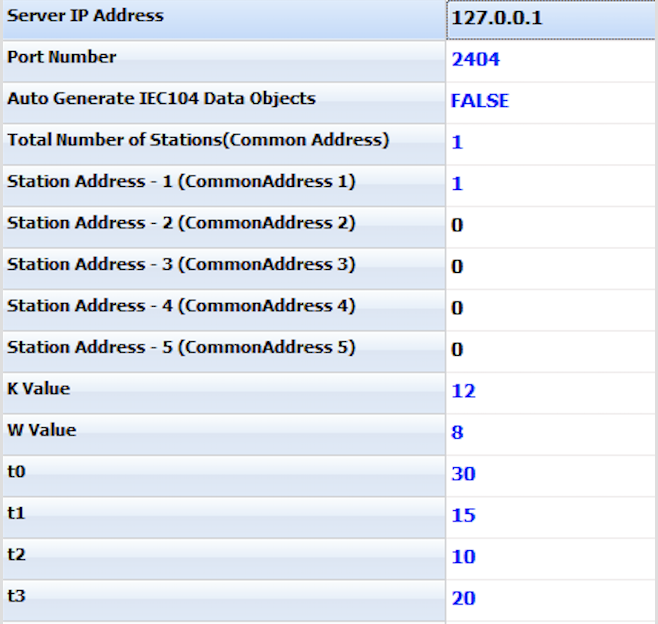
\includegraphics{IEC-Configuration}}
    \caption{Defaultná konfigurácia nového klienta}
    \label{ClientConf}
    \end{minipage}
    \begin{minipage}[b]{0.4\textwidth}
    \centering
    \scalebox{0.52}{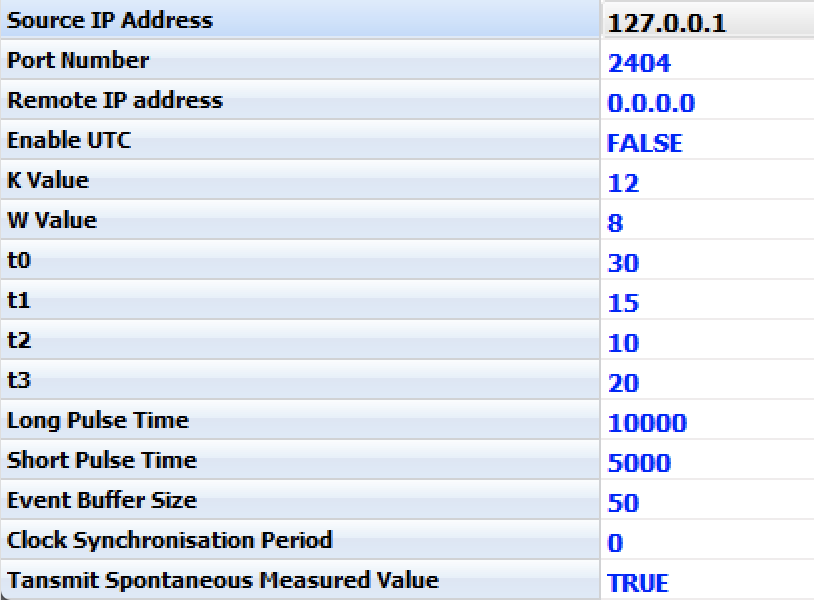
\includegraphics{IECS-Configuration}}
    \caption{Defaultná konfigurácia nového servera}
    \label{ServerConf}
    \end{minipage}
\end{figure} \par
Vytvorenie spojenia a testovanie programov pozostávalo z niekoľkých krokov:
\begin{enumerate}
\item Spustenie programu servera
\item Kliknutie na {\tt Add Server}
\item Komunikácia prebiehala na rozhraní loopback, nebolo treba nič nastavovať čo sa týka spojenia
\item {\tt Configuration} $\rightarrow$ {\tt Add Row}:
\begin{itemize}
\item {\tt Group} $\rightarrow$ {\tt Measured Short Float}
\item {\tt Type Id} $\rightarrow$ {\tt M\_ME\_NC\_1 = 13}
\item {\tt Starting IOA} $\rightarrow$ 1
\item {\tt Range} $\rightarrow$ 5
\end{itemize}
\item {\tt Add Row}
\begin{itemize}
\item {\tt Group} $\rightarrow$ {\tt Set Point Command - Float Value}
\item {\tt Type Id} $\rightarrow$ {\tt C\_SE\_NC\_1 = 50}
\item {\tt Starting IOA} $\rightarrow$ 10
\item {\tt Range} $\rightarrow$ 5
\end{itemize}
\item {\tt Load Configuration}
\item {\tt Data\_Objects}
\item Následne bolo potrebné všetky objekty typu {\tt Set Point} (začínajúce číslom 10) namapovať na objekty uchovávajúce namerané hodnoty:
\begin{enumerate}
\item Pravý klik na objekt
\item {\tt Map}
\item V zozname vybrať objekt na ktorý sa ide mapovať, ideálne 10 $\rightarrow$ 1, atp.
\end{enumerate}
\item {\tt Start Communication}
\item Spustenie programu klienta
\item {\tt Add Client}
\item Nebolo potrebné nastavovať IP adresu, ani port, komunikácia prebiehala na rozhraní loopback na štandardnom porte 2404
\item {\tt Data\_Objects} $\rightarrow$ {\tt Start Communication}
\item Klient sa pripojil k serveru a zobrazil pripojené objekty
\end{enumerate}
Po kliknutí pravým tlačítkom na jednotlivé objekty sa zobrazili príkazy, ktoré bolo možné zasielať serveru. {\tt Point Command} na vzdialené nastavenie hodnôt, {\tt Station Commands} na zaslanie štandardných príkazov typu {\tt General Interrogation}, {\tt Counter Interrogation}, {\tt Directory Read} atp. Priebeh komunikácie je možné vidieť v logovacej správe, ktorá je automaticky generovaná oboma programami. Správu je možné zobraziť po rozkliknutí záložky {\tt Log}. \par
Testovanie spočívalo v zaslaní niekoľkých štandardných príkazov medzi klientom a serverom na overenie, že komunikácia odpovedá štandardom protokolu IEC 60870-5-104. Zaslané príkazy boli zamerané hlavne na vzdialené čítanie a nastavenie hodnôt. Na obrázku \ref{iectopology} je ukázaná topológia použitá pri testovaní. 
\begin{figure}[h]
    \centering
    \scalebox{0.8}{\includegraphics{iec_topology}}
    \caption{Ukážka testovacej topológie programov Client/Server Simulator}
\label{iectopology}
\end{figure}
Programy boli spustené na jednom zariadení. Komunikácia bola zachytávaná pomocou nástroja RawCap na rozhraní loopback. Zachytená komunikácia je v súbore C/SSimulator.pcap, ktorý je uložený v github repozitári \footnote{GitHub \url{https://github.com/janpristas/bakalarska-praca}}. \par
\noindent \textbf{Zhrnutie:} Client/Server Simulator programy sú asi najprehladnejšie varianty s najväčšou škálou možností na emuláciu prevádzky SCADA systémov využívajúcich protokol IEC 60870-5-104. Veľkou nevýhodou ale zostáva, že demoverzie, s ktorými som pracoval, poskytujú iba 15 minút na prácu a následne sa vypnú. Celý systém je potom nutné konfigurovať odznova.

\subsection{QTester 104}
\textbf{Výrobca:} Autorom produktu je Ricardo Olsen, majiteľ spoločnosti DSC Systems. Jeho prácou je konfigurácia a vývoj riadiacich systémov pre komunikáciu klient/server. \par
\noindent \textbf{Popis produktu:} QTester 104 je open source software, ktorý slúži na získavanie dát z koncových staníc a ich riadenie. Je možné si ho zdarma stiahnuť na stránke {\tt sourceforge.net}\footnote{QTester 104 \url{https://sourceforge.net/projects/qtester104/} [Online: Október 2017]}. Umožňuje sledovať stav koncových zariadení, sťahovať z nich dáta a posielať príkazy. Pracuje iba ako klient(master). Je vytvorený v C++ za pomoci QT. Záznam komunikácie je možné uložiť vo forme textového dokumentu. Software je iba časťou väčšieho HMI projektu\footnote{OSHMI \url{https://sourceforge.net/projects/oshmiopensubstationhmi/} [Online: November 2017]} a slúži ako modul pre HMI. Môže byť ale použitý aj samostatne ako protokol tester. \par
\noindent \textbf{Protokoly:} Program využíva na komunikáciu protokol IEC 60870-5-104. \par
\noindent \textbf{Zariadenia:} Kedže QTester 104 funguje iba ako klient, nie je schopný emulovať koncové zariadenia. Je možné ale pripojiť reálne, alebo iným programom emulované zariadenia. Komunikácia prebieha cez TCP/IP spojenie. \par
\noindent \textbf{Typ:} Program je open source a je spolu so zdrojovými kódmi voľne k dispozíci. Taktiež ho je možné voľne distribuovať ďalej. \par
\noindent \textbf{Platforma:} S programom je možné pracovať pod OS Windows a Linux. Na obrázku \ref{QTester} je ukážka užívateľského rozhrania programu. \par
\begin{figure}[h]
	\centering
    \scalebox{0.35}{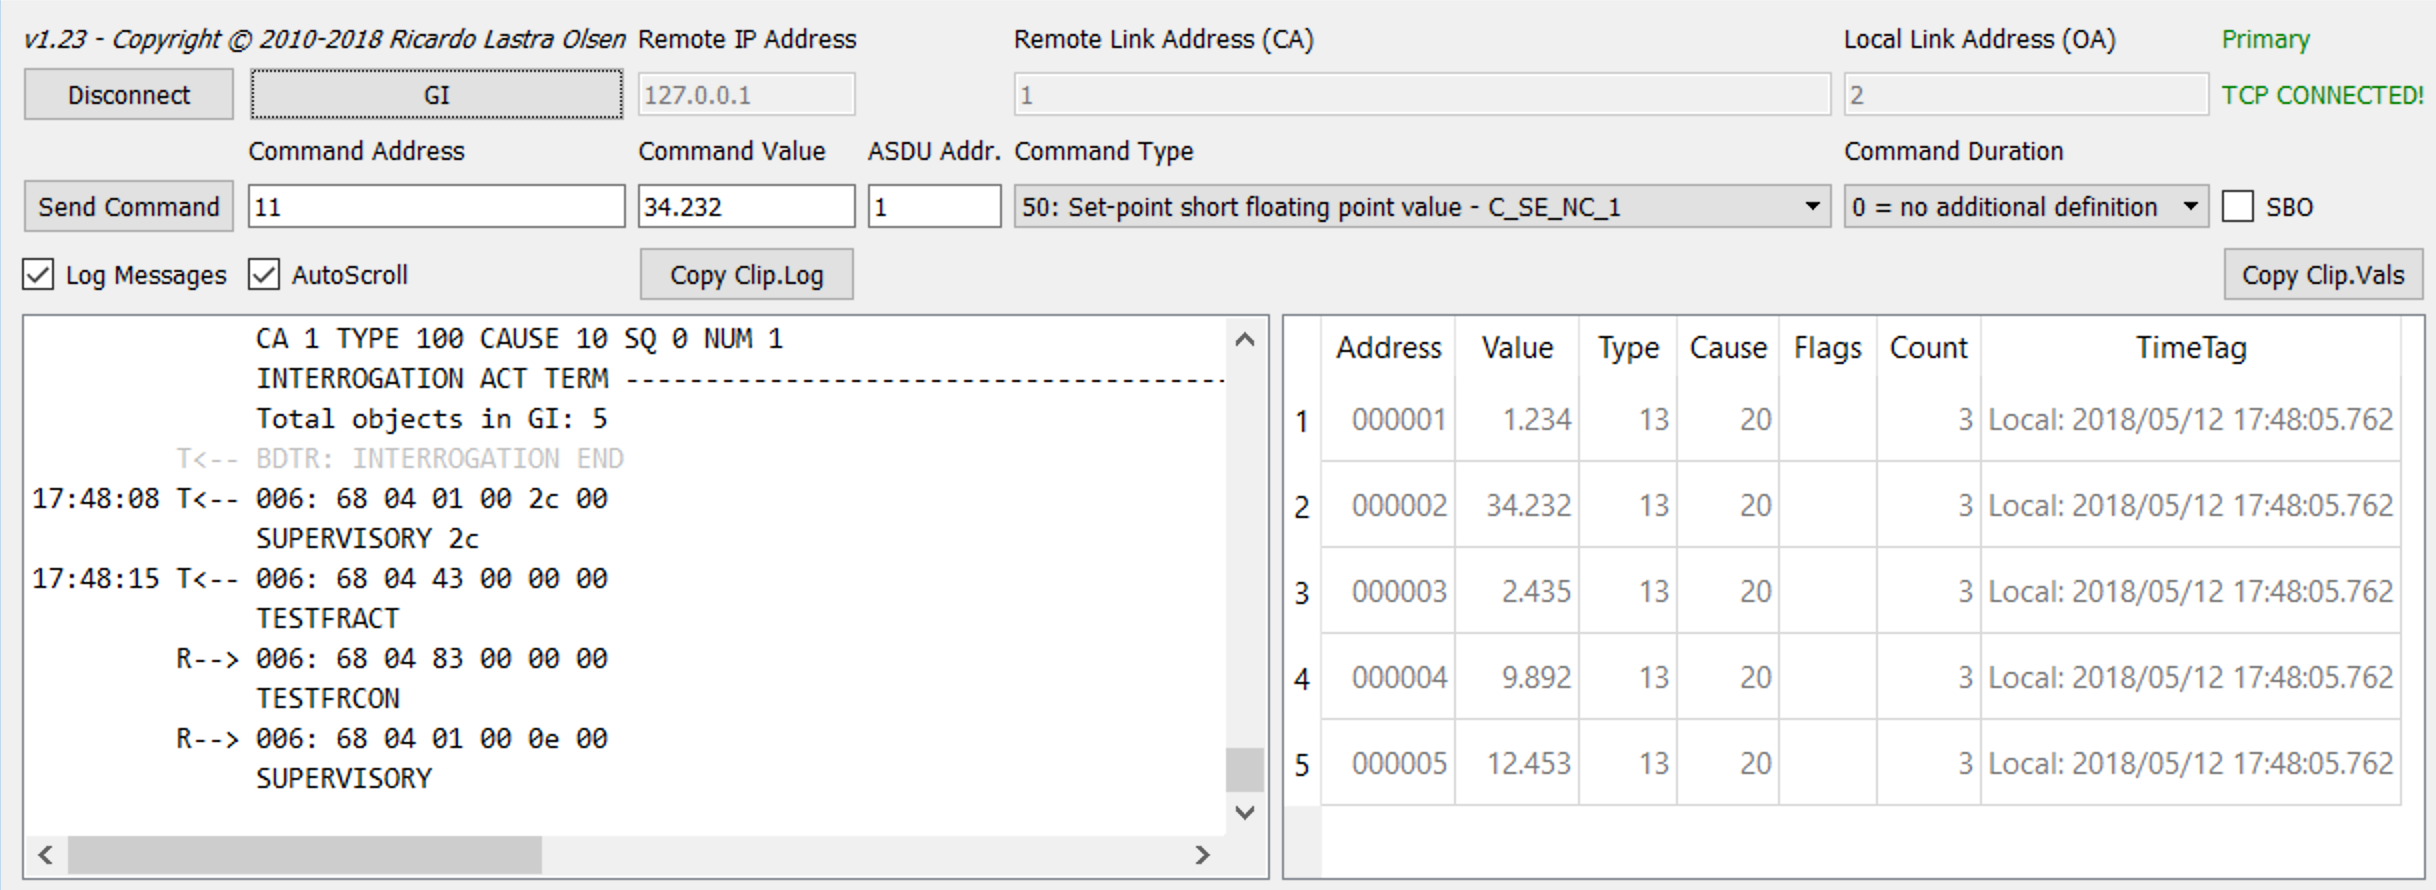
\includegraphics{QTester}}
    \caption{Ukážka užívateľského rozhrania programu QTester 104}
\label{QTester}
\end{figure}
\noindent \textbf{Prípadová štúdia:} QTester 104 umožňuje v rámci monitorovania mať vytvorenú iba jednú stanicu pre klienta, čo je vlastne program samotný, a umožňuje pripojenie jednej stanice servera. Testovanie prebiehalo pod OS Windows za pomoci programu IEC 104 Server Simulator, ktorý bol popísaný v predchádzajúcej podkapitole. \par
Vytvorenie testovacej topológie prebiehalo v niekoľkých krokoch:
\begin{enumerate}
\item Spustenie a konfigurácia servera, rovnako ako v predchádzajúcej podkapitole
\item Spustenie programu QTester 104: {\tt qtester104} $\rightarrow$ {\tt bin} $\rightarrow$ {\tt QTester104}
\item Pri testovaní bolo použité rozhranie loopback na ktorom sa program ihneď po spustení snažil spojiť so serverom, nebola potrebná dodatočná konfigurácia
\item Po úspešnom spojení, kliknúť na {\tt GI (General Interrogation)} aby sa načítali objekty pripojené k serveru
\item Zakliknúť {\tt Log Messages}, prípadne {\tt AutoScroll} na zobrazenie logovacej správy
\end{enumerate}
Po úspešnej konfigurácií a prepojení je možné zasielať serveru príkazy. Pre zaslanie príkazu je potrebné nastaviť niekoľko hodnôť:
\begin{itemize}
\item {\tt Command Address}, adresa {\tt Set-point} objektu namapovaného na objekt, ktorý chceme nastaviť, napr. 10
\item {\tt Command Value}, hodnota na ktorú chceme objekt nastaviť, musí byť typu čísla s pohyblivou rádovou čiarkou, napr 123.456
\item {\tt ASDU address}, hodnotu nastaviť na 1
\end{itemize} \par
Práca s programom je vo všeobecnosti veľmi intuitívna, po spustení stačí iba zadať IP adresu servera, program sa s ním automaticky spojí a je možné s ním ihneď pracovať. Na obrázku \ref{QTester104} je ukážka stavu programu ihneď po spustení.
\begin{figure}[h]
    \centering
    \scalebox{0.43}{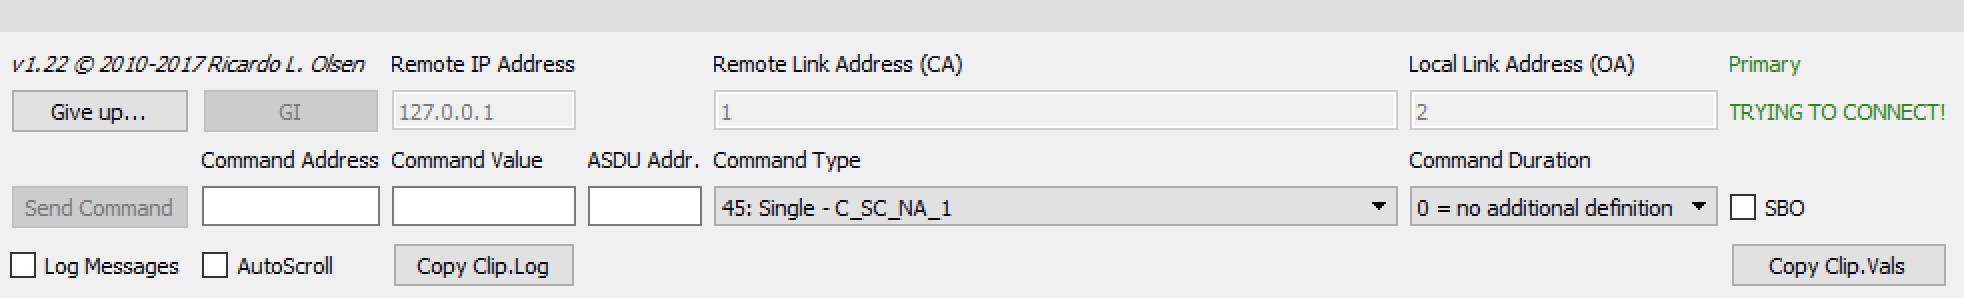
\includegraphics{QTester104}}
    \caption{Defaultné nastavenie programu pri spustení}
\label{QTester104}
\end{figure}
Pri každej zmene hodnôt na strane servera sú automaticky aktualizované v QTestery. Pri testovaní bolo vytvorených päť koncových zariadení typu {\tt M\_ME\_TF} na zaznamenávanie hodnôt s pohyblivou rádovou čiarkou. Topológiu je možné vidieť na obrázku \ref{QT-Topology}.
\begin{figure}[h]
    \centering
    \scalebox{0.8}{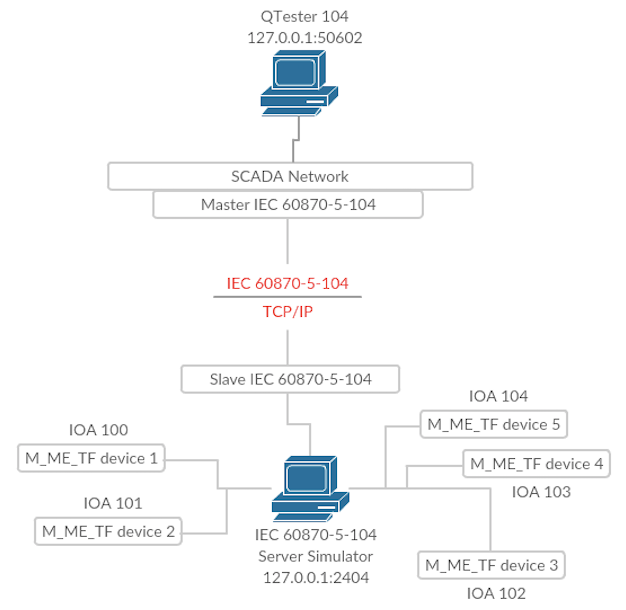
\includegraphics{QT-Topology}}
    \caption{QTester 104 - Testovacia topológia}
\label{QT-Topology}
\end{figure}
Oba programy boli spustené na jednom zariadení a komunikácia medzi nimi bola následne odchytávaná v nástroji RawCap na rozhraní loopback. Z komunikácie bol vygenerovaný súbor QTester104.pcap uložený v github repozitári \footnote{GitHub \url{https://github.com/janpristas/bakalarska-praca}}. \par
\noindent \textbf{Zhrnutie:} QTester 104 je celkom prepracovaný a užívateľsky prívetivý monitorovací nástroj. Výhodou je, že je open source a je možné s ním voľne pracovať a distribuovať ho. Ďalšiu výhodu vidím v jednoduchom a intuitívnom GUI v ktorom sa veľmi dobre pracuje. Nevýhodou je menšia škála možností oproti programu Client Simulator z predchádzajúcej kapitoly, na testovacie účely bol ale postačujúci.

\section{Zhrnutie}
\tab V tejto kapitole bol uvedený základný prehľad priemyselných monitorovacích a emulačných nástrojov pre SCADA systémy. Bola popísaná najmä ich základná funkcionalita a schopnosť komunikácie odpovedajúcej patričným štandardom. \par
\subsection{DLMS/COSEM}
\par
\begin{tcolorbox}[enhanced, title={Porovnanie emulátorov pre protokol DLMS/COSEM}, clip upper, fontupper=\sffamily,%
    tabularx={>{\cellcolor[gray]{.5}\color{white}}r%
              >{\centering\arraybackslash}X%
              >{\centering\arraybackslash}X}]
  &\cellcolor{black!80}\color{white} DLMS Director   &\cellcolor{black!80}\color{white} XmlDemo \\
Platforma       & OS Windows                         & OS Windows \\
Klient/Server   & Klient                             & Klient \\
Kom. protokoly  & TCP/IP, HDLC                       & TCP/IP, HDLC iba cez sériovú linku \\
Licencia        & Open Source                        & Open Source \\
Vlastná konfig. & Nie, iba objekty pripojené k serveru & Nie, iba objekty pripojené k serveru \\
GUI             & Veľmi dobré a intuitívne           & Veľmi jednoduché \\
Celkový dojem   & Dobre spracovaný program s veľkou škálou možností  & Dobre spracovaný program podporujúci základnú potrebnú funkčnosť
\end{tcolorbox} \par 
Pre protokol DLMS/COSEM boli popísané programy DLMS Director a XmlDemo. Oba programy sú dobre spracované a poskytujú potrebnú funkčnosť a umožňujú vytvoriť komunikáciu odpovedajúcu štandardu DLMS/COSEM, avšak program DLMS Director poskytuje navrch možnosť komunikácie pomocou HDLC, väčšiu škálu možných nastavení a taktiež má oveľa prívetivejšie a intuitívnejšie GUI. Pre protokol DLMS/COSEM budem ďalej využívať program DLMS Director.

\subsection{IEC 60870-5-104}
\par
\begin{tcolorbox}[enhanced, title={Porovnanie emulátorov pre protokol IEC 104, 1. časť}, clip upper, fontupper=\sffamily,%
    tabularx={>{\cellcolor[gray]{.5}\color{white}}r%
              >{\centering\arraybackslash}X%
              >{\centering\arraybackslash}X}]
  &\cellcolor{black!80}\color{white} WinPP104   &\cellcolor{black!80}\color{white} Knižnica OpenMUC - j60870 \\
Platforma               & OS Windows            & OS Windows/Unix like OS \\
Klient/Server           & Klient/Server         & Klient/Server \\
Kom. protokoly          & TCP/IP                & TCP/IP \\
Licencia                & Demoverzia           & Licencovaná pod GPLv3 \\
Vlastná konfig.         & Možnosť konfigurácie vlastných šablón správ & Možnosť vytvoriť si vlastný program klient/server podľa potreby užívateľa \\
GUI                     & Trochu komplikované   & Vzorové programy bez GUI, iba ako terminálové aplikácie \\
Celkový dojem           & Program je relatívne náročný na prvotné zorientovanie a pochopenie, taktiež je nevýhodou obmedzenie demoverzie na zaslanie/prijatie iba 20 správ & Vzorové programy jednoduché (slúžia iba na ilustráciu možností knižnice), knižnica je dobre spracovaná, umožňuje veľkú škálu možností na tvorbu vlastných staníc
\end{tcolorbox}

\begin{tcolorbox}[enhanced, title={Porovnanie emulátorov pre protokol IEC 104, 2. časť}, clip upper, fontupper=\sffamily,%
    tabularx={>{\cellcolor[gray]{.5}\color{white}}r%
              >{\centering\arraybackslash}X%
              >{\centering\arraybackslash}X}]
  &\cellcolor{black!80}\color{white} Client/Server Simulator &\cellcolor{black!80}\color{white} QTester 104 \\
Platforma   & OS Windows, možnosť získať SDK pre klienta a server od výrobcu na OS Windows/Linux & OS Windows/Linux \\
Klient/Server   & Klient/Server & Klient \\
Kom. protokoly    & TCP/IP & TCP/IP \\
Licencia & Demoverzia & Open Source \\
Vlastná konfig. & Nie, možnosť využívať iba štandardné objekty & Nie, iba objekty pripojené k serveru \\
GUI    & Dobre spracované, miestami trochu komplikované & Veľmi dobré, jednoduché a intuitívne \\
Celkový dojem   & Veľmi dobre spracované programy s veľkou škálou možností, nevýhodou je obmedzenie na 15 minút pri demoverzií & Veľmi dobre spracovaný program, veľmi jednoduchý, podporujúci základnú požadovanú funkcionalitu
\end{tcolorbox} \par
Pre protokol IEC 60870-5-104 boli popísané programy WinPP104, QTester 104, IEC 60870-5-104 Client/Server Simulator a knižnica pre jazyk Java OpenMUC - j60870. Každý z programov poskytuje inú funkcionalitu a škálu možností konfigurácie. Všetky programy umožňujú vytvoriť komunikáciu odpovedajúcu štandardu IEC 60870-5-104. Užívateľsky najprívetivejšie a pre ďalšie testovanie sú najvhodnejšie programy Client/Server Simulátor a QTester 104. Programy podporujú veľkú škálu možností na konfiguráciu staníc a špecifikáciu komunikácie. Taktiež poskytujú veľmi intuitívne prostredie a pracuje sa s nimi jednoducho. Oproti tomu je program WinPP104 oveľa komplikovanješí a práca s ním nie je jednoduchá. \par 
Rovnako komplikovaná je práca s knižnicou OpenMuc - j60870, ktorá síce umožňuje vytvorenie vlastného programu klient/server, vyžaduje však vyššiu znalosť programovacieho jazyka Java a problematiky samotnej. Výhodou programu QTester 104 je jeho voľná dostupnosť a kvalitné spracovanie. Nevýhodou ale zostáva možnosť vytvorenia spojenia iba medzi jedným klientom a serverom. Tento problém riešia programy IEC 60870-5-104 Client/Server Simulator, ktoré umožňujú vytvorenie väčšej~topológie. Avšak nevýhodou demoverzie je časové obmedzenie, ktoré umožňuje s programami pracovať maximálne 15 minút. \par
V praktickej časti svojej práce budem vychádzať z programov DLMS Director, QTester 104 a IEC 60870-5-104 Client/Server Simulator.